%
%===============>>  ГРУППА 11-4 МОДУЛЬ 3 <<=============
%
\setmodule{3}
%
%===============>>  Занятие 1  <<===============
%
\begin{class}[number=1]
	\begin{listofex}
		\item
		\begin{minipage}[t]{0.67\textwidth}
			На рисунке изображен график функции \( f(x)=kx+b \). Найдите \( f(-9) \).
		\end{minipage}
		\begin{minipage}[c]{0.2\textwidth}
			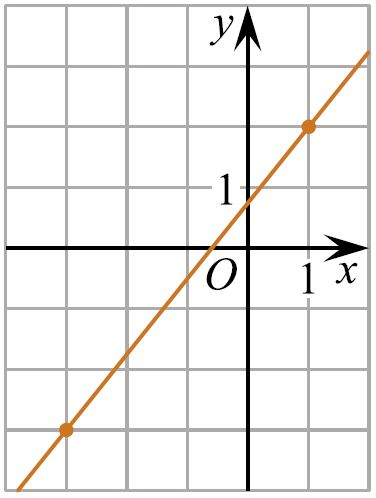
\includegraphics[align=t, width=0.8\textwidth]{../pics/G112M3C2-1}
		\end{minipage}
		\item
		\begin{minipage}[t]{0.67\textwidth}
			На рисунке изображены графики двух линейных функций. Найдите абсциссу точки пересечения графиков.
		\end{minipage}
		\begin{minipage}[c]{0.2\textwidth}
			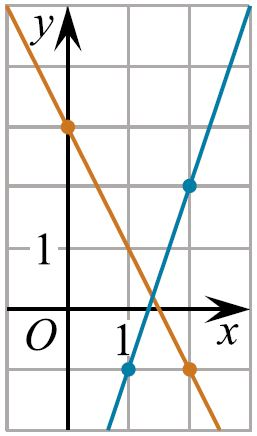
\includegraphics[align=t, width=0.8\textwidth]{../pics/G112M3C2-2}
		\end{minipage}
		\item
		\begin{minipage}[t]{0.57\textwidth}
			На рисунке изображен график функции \( f(x)=\dfrac{x^2}{a}+bx+c \). Найдите \( f(3,5) \).
		\end{minipage}
		\begin{minipage}[c]{0.3\textwidth}
			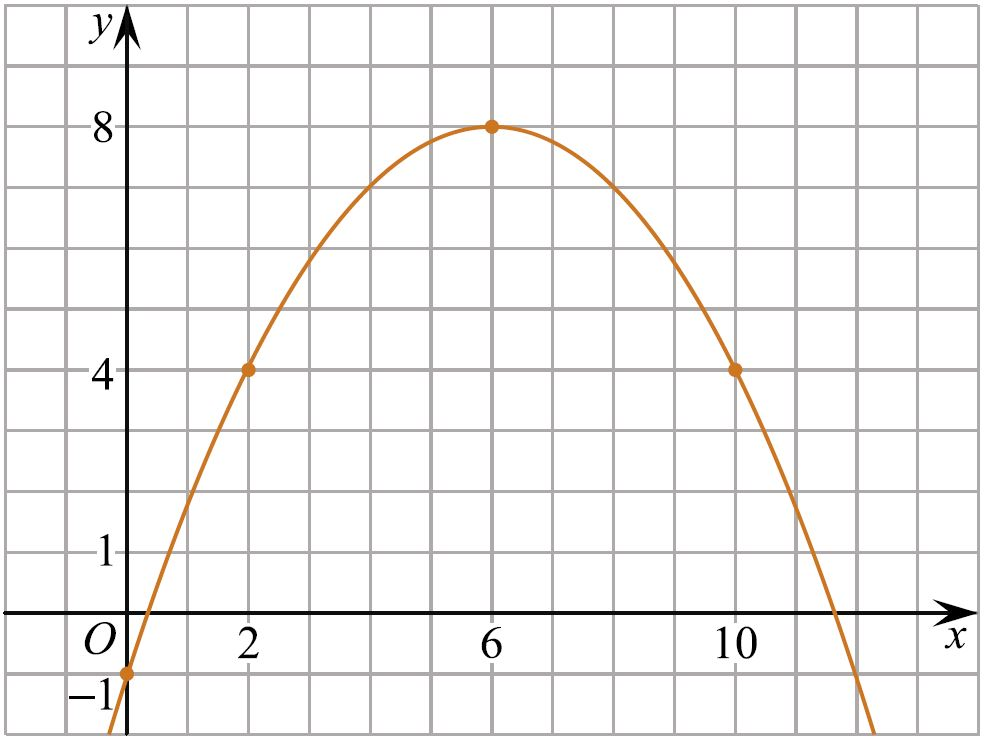
\includegraphics[align=t, width=\textwidth]{../pics/G112M3C2-3}
		\end{minipage}
		\item
		\begin{minipage}[t]{0.57\textwidth}
			На рисунке изображен график функции \( f(x)=\dfrac{x^2}{a}+bx+c \). Найдите \( f(4) \).
		\end{minipage}
		\begin{minipage}[c]{0.3\textwidth}
			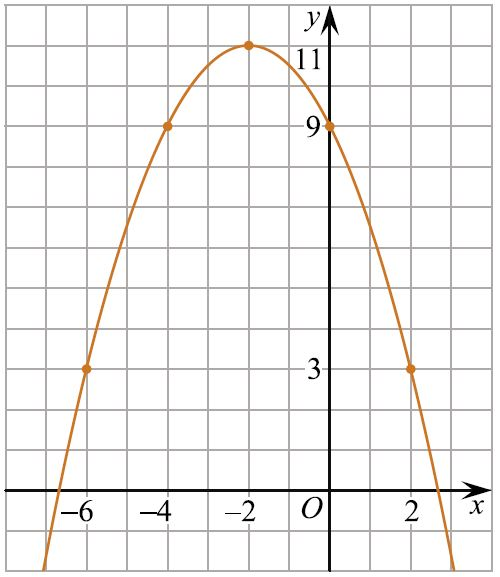
\includegraphics[align=t, width=\textwidth]{../pics/G112M3C2-4}
		\end{minipage}
		\item
		\begin{minipage}[t]{0.57\textwidth}
			На рисунке изображен график функции \( f(x)=\dfrac{k}{x}+a \). Найдите, при каком значении \( x \) значение функции будет равно \( 0,8 \).
		\end{minipage}
		\begin{minipage}[c]{0.3\textwidth}
			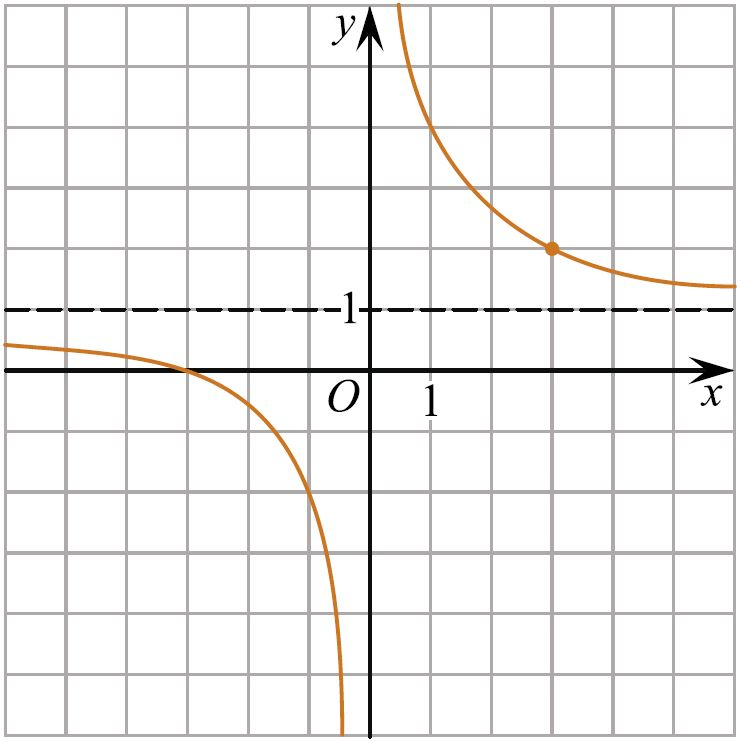
\includegraphics[align=t, width=\textwidth]{../pics/G112M3C2-5}
		\end{minipage}
		\item
		\begin{minipage}[t]{0.57\textwidth}
			На рисунке изображены графики функций \( f(x)=2x^2+11x+11 \) и \( y=ax^2+bx+c \), которые пересекаются в точках \( A \) и \( B \). Найдите абсциссу точки \( B \).
		\end{minipage}
		\begin{minipage}[c]{0.3\textwidth}
			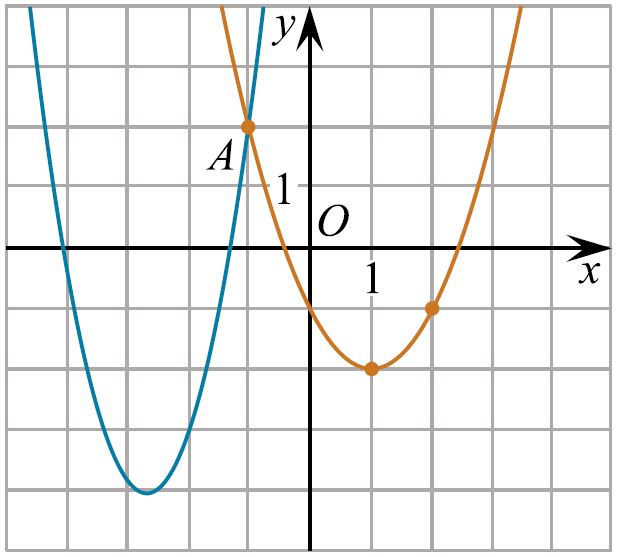
\includegraphics[align=t, width=\textwidth]{../pics/G112M3C2-6}
		\end{minipage}
		\item Велосипедист выехал с постоянной скоростью из города \( A \) в город \( B \), расстояние между
		которыми равно \( 70 \) км. На следующий день он отправился обратно в \( A \) со скоростью на \( 3 \) км/ч больше прежней. По дороге он сделал остановку на \( 3 \) часа. В результате велосипедист затратил на обратный путь столько же времени, сколько на путь из \( A \) в \( B \). Найдите скорость велосипедиста на пути из \( B \) в \( A \). Ответ дайте в км/ч.
		\item В сосуд, содержащий \( 5 \) литров \( 12 \)--процентного водного раствора некоторого вещества,
		добавили \( 7 \) литров воды. Сколько процентов составляет концентрация получившегося раствора?
		\item При производстве в среднем на каждые \( 2982 \) исправных насоса приходится \( 18 \) неисправных.
		Найдите вероятность того, что случайно выбранный насос окажется неисправным.
	\end{listofex}
\end{class}
%
%===============>>  Занятие 2  <<===============
%
%\begin{class}[number=2]
%	\begin{listofex}
%		\item Пусто
%	\end{listofex}
%\end{class}
%
%===============>>  Домашняя работа 1  <<===============
%
%\begin{homework}[number=1]
%	\begin{listofex}
%		\item Пусто
%	\end{listofex}
%\end{homework}
%
%===============>>  Занятие 3  <<===============
%
%\begin{class}[number=3]
%	\begin{listofex}
%		\item Пусто
%	\end{listofex}
%\end{class}
%
%===============>>  Занятие 4  <<===============
%
%\begin{class}[number=4]
%	\begin{listofex}
%		\item Пусто
%	\end{listofex}
%\end{class}
%
%===============>>  Домашняя работа 2  <<===============
%
%\begin{homework}[number=2]
%	\begin{listofex}
%		\item Пусто
%	\end{listofex}
%\end{homework}
%
%===============>>  Занятие 5  <<===============
%
%\begin{class}[number=5]
%	\begin{listofex}
%		\item Пусто
%	\end{listofex}
%\end{class}
%
%===============>>  Занятие 6  <<===============
%
%\begin{class}[number=6]
%	\begin{listofex}
%		\item Пусто
%	\end{listofex}
%\end{class}
%
%===============>>  Домашняя работа 3  <<===============
%
%\begin{homework}[number=3]
%	\begin{listofex}
%		\item Пусто
%	\end{listofex}
%\end{homework}
%
%===============>>  Занятие 7  <<===============
%
\title{Подготовка к проверочной работе}
	\begin{listofex}
		\item Изюм получается в процессе сушки винограда. Сколько килограммов винограда потребуется для получения \( 82 \) килограммов изюма, если виноград содержит \( 90\% \) воды, а изюм содержит \( 5\% \) воды?
		\item Смешали \( 3 \) литра \( 35 \)-процентного водного раствора некоторого вещества с \( 12 \) литрами \( 15 \)-процентного водного раствора этого же вещества. Сколько процентов составляет концентрация получившегося раствора?
		\item Имеется два сплава. Первый содержит \( 10\% \) никеля, второй -- \( 35\% \) никеля. Из этих двух сплавов получили третий сплав массой \( 250 \) кг, содержащий \( 25\% \) никеля. На сколько килограммов масса первого сплава была меньше массы второго?
		\item Из городов \( A \) и \( B \), расстояние между которыми равно \( 330 \) км, навстречу друг другу одновременно выехали два автомобиля и встретились через \( 3 \) часа на расстоянии \( 180 \) км от города \( B \). Найдите скорость автомобиля, выехавшего из города \( A \). Ответ дайте в км/ч.
		\item Иван и Алексей договорились встретиться в Н-ске. Они едут к Н-ску разными дорогами. Иван звонит Алексею и узнаёт, что тот находится в \( 168 \) км от Н-ска и едет с постоянной скоростью \( 72 \) км/ч. Иван в момент звонка находится в \( 165 \) км от Н-ска и ещё должен по дороге сделать \( 30 \)-минутную остановку. С какой скоростью должен ехать Иван, чтобы прибыть в Н-ск одновременно с Алексеем?
		\item Два гонщика участвуют в гонках. Им предстоит проехать 46 кругов по кольцевой трассе протяжённостью \( 4 \) км. Оба гонщика стартовали одновременно, а на финиш первый пришёл раньше второго на \( 5 \) минут. Чему равнялась средняя скорость второго гонщика, если известно, что первый гонщик в первый раз обогнал второго на круг через \( 60 \) минут? Ответ дайте в км/ч.
		\item 
	\end{listofex}
%
%===============>>  Проверочная работа  <<===============
%
%\begin{exam}
%	\begin{listofex}
%		\item Пусто
%	\end{listofex}
%\end{exam}
\begin{consultation}
	\begin{listofex}
		\item Найти производные функций:
		\begin{enumcols}[itemcolumns=2]
			\item \( y=x^4-2x+1 \)
			\item \( y=3\sqrt[3]{x^2}+2x^3\sqrt{x}+\dfrac{1}{x^3} \)
			\item \( y=\dfrac{x^3-2x^2+1}{x-1} \)
			\item \( y=\dfrac{1-\cos2x}{1+\cos2x} \)
			\item \( y=e^{x^3-5x^2} \)
			\item \( y=\sin2x\tg x \)
		\end{enumcols}
		\item Вычислить значения производной функции при указанном значении переменной:
		\begin{enumcols}[itemcolumns=3]
			\item \( f(x)=\dfrac{x^2-2}{x^2+2};\;f'(2) \);
			\item \( f(x)=\dfrac{x}{3}-\dfrac{3}{x};\;f'(3) \);
			\item \( f(x)=\dfrac{\cos x}{1+\sin x};\;f'\left( \dfrac{\pi}{2} \right) \).
		\end{enumcols}
		\item Найти точку максимума функции \( y=7+12x-x^3 \). \answer{\( 2 \)}
		\item Найти наибольшее значение функции \( y=x^3+2x^2+x+\sin\left( \dfrac{\pi}{6} \right) \) на отрезке \( [-4;-1] \). \answer{\( 3 \)}
		\item Найти точку максимума функции \( y=-\dfrac{x}{x^2+289} \). \answer{\( -17 \)}
		\item Найдите наименьшее значение функции \( y=3+\dfrac{5\pi}{4}-5x-5\sqrt{2}\cos x \) на отрезке \( \left[ 0;\dfrac{\pi}{2} \right] \). \answer{\( -2 \)}
		\item Найдите наименьшее значение функции \( y=\sqrt{x^2-6x+13} \). \answer{\( 2 \)}
	\end{listofex}
\end{consultation}